\chapter{Versicherung}
\label{chap:Versicherung}
Im Bereich Versicherung gibt es mehrere Bestrebungen, mithilfe von Smart Contracts die automatische Abwicklung von Versicherungsfällen zu regeln. Die 2018 gegründete B3i Initiative, hinter der namhafte Versicherungsunternehmen wie Zurich, AXA, Generali und die Allianz stehen, hat sich zur Aufgabe gemacht, Standards für die Branche zu entwickeln und das nötige Netzwerk und die Anwendungen aufzubauen \cite[vgl.][]{B3iWhoWeAre2019}. Da die Applikation erst im Juli 2019 startet \cite[vgl.][]{B3iHackathon2019}, eignet es sich nicht, um tiefer darauf einzugehen.

Eine bereits lauffähige Anwendung auf der Ethereum Blockchain existiert mit fizzy, einer Applikation von AXA. Fizzy sichert Personen gegen Flugzeugverspätungen bei mehr als zwei Stunden oder kompletter Annulierung des Fluges ab. Mit Anlegen einer Versicherung, was bis spätestens fünf Tage vor Abflug möglich ist, wird die Fluginformation an einen Smart Contract weitergegeben, welcher die Daten in der Blockchain speichert. Durch eine Koppelung an Flugdaten wird der Betrag im Versicherungsfall innerhalb einer Standard-Bankenlaufzeit ausbezahlt. Die Gebühren für die Absicherung werden dabei von einem Algorithmus anhand des Flug-Ausfallsrisikos berechnet. Durch den Einsatz von Blockchain-Technologie wird auf beiden Seiten Transparenz und Unveränderlichkeit der Bedingungen garantiert. \cite[vgl.][]{Fizzy2019}

Da fizzy mit \cite{Clement2019} einen Artikel bereitgestellt hat, um einen besseren Einblick in den zugrundeliegenden Smart Contract zu bekommen, wird im Folgenden ein Beispiel besprochen.\\
Seit 22. Mai 2019 gibt es eine neue Variante des Smart Contracts \cite{EtherscanNewContract2019}, welcher mit 742 Zeilen Solidity Code deutlich mehr Funktionalität liefert, als der ursprüngliche Smart Contract mit gerade einmal etwas mehr als 200 Codezeilen \cite{EtherscanOldContract2019}. Zur Betrachtung wird nun in Teilen der neue Contract herangezogen.

Die Schritte (1) und (5) aus Abbildung \ref{fig:fizzyAblauf} können vernachlässigt werden, da sie sich nur mit der Eingabe der persönlichen Daten und Flugdetails beschäftigen und der letzendlichen Kompensation im Versicherungsfall dienen. Interessanter sind hier die Schritte (2), (3) und (4), welche sich direkt mit dem Smart Contract beschäftigen. Nach diesen wird jeweils die Funktion \texttt{InsuranceUpdate(...)} im Nachgang aufgerufen.\clearpage

\begin{figure}[h!]
  \centering
  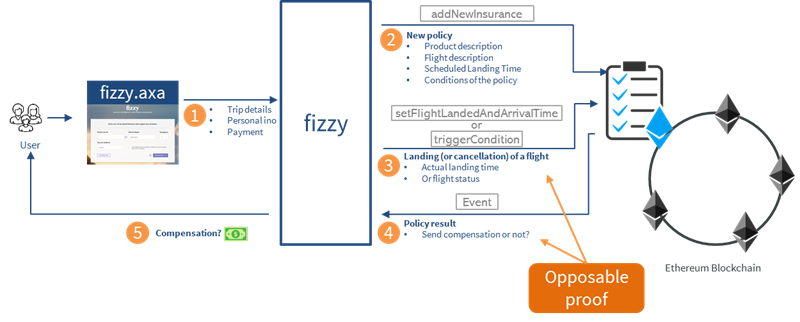
\includegraphics[width=\textwidth]{Bilder/fizzyAblauf.png}
  \caption[Ablauf fizzy Smart Contract]{Ablauf fizzy Smart Contract \cite{Clement2019}}
  \label{fig:fizzyAblauf}
\end{figure}

Anfangs muss eine Versicherung angelegt werden. Dafür steht die Solidity-Funktion \texttt{addNewInsurance(bytes32 flightId, uint256 productId, uint256 premium, uint256 indemnity, uint256 limitArrivalTime, uint256 conditions)} bereit. Kurz zur Erläuterung der einzelnen Parameter:

\begin{itemize}
    \item \texttt{flightId}: In Hexadezimal-Darstellung steht die Flugnummer inklusive Abflugdatum (UNIX-Timestamp) bereit
    \item \texttt{productId}: Identifikator, um Versicherung eindeutig zu kennzeichnen; es können auch mehrere Versicherungen mit der gleichen \texttt{flightId} existieren
    \item \texttt{premium}: Prämienbetrag, hexadezimal codiert
    \item \texttt{indemnity}: Entschädigung, hexadezimal codiert
    \item \texttt{limitArrivalTime}: spätester Ankunftszeitpunkt, d.h. geplanter Ankunftszeitpunkt + 2 Stunden (UNIX-Timestamp, UTC)
    \item \texttt{conditions}: binär kodierte Konditionen; 1001 (2) = 9 (10): für Verspätung und Canceln abgesichert, 0001 (2) = 1 (10): nur für Canceln abgesichert
\end{itemize}

Aus dem Contract wird die Transaktion\\
\texttt{0x6ecc9789935ff5c518f44fa9b2601f40ac6a8a4fa45f16f21146251dc9c9536a} beispielhaft ausgewählt. Die zugehörigen Werte obiger Funktion sind in Abbildung \ref{fig:fizzyNewInsurance} zu sehen.

\begin{figure}[h!]
  \centering
  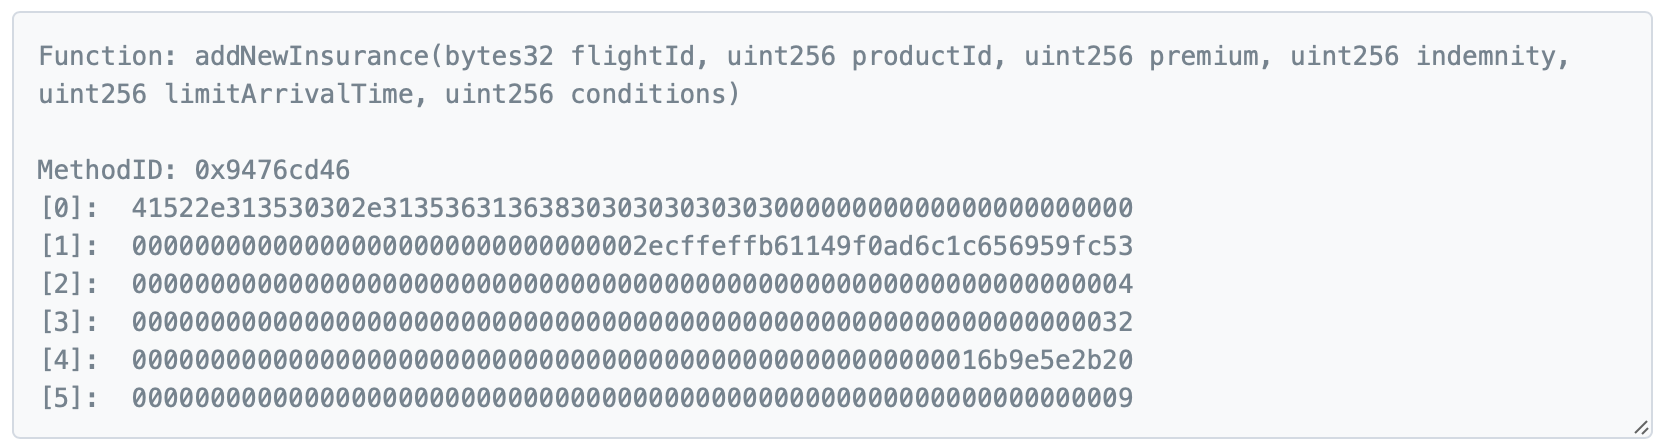
\includegraphics[width=\textwidth]{Bilder/FizzyExampleNewInsurance.png}
  \caption[Input-Daten addNewInsurance]{Input-Daten addNewInsurance \cite{FizzyNewInsurance2019}}
  \label{fig:fizzyNewInsurance}
\end{figure}

Mithilfe eines Hexadezimal zu String Decoders lässt sich die \texttt{flightId} zu \\ \texttt{AR.1500.1561680000000} umwandeln. Dabei beschreibt \texttt{AR.1500} den Flug, was sich nach einer Suchmaschinen-Recherche als Reise von Buenos Aires nach Córdoba mit der Fluggesellschaft Aerolineas Argentinas herausstellt. \texttt{1561680000000} ergibt mit einem UNIX-Timestamp-Converter den 28. Juni 2019. Auch die Hexadezimalen Werte der Prämien- und Entschädigungsbeträge lassen sich einfach umwandeln. So kommt man auf eine Prämie von 4€ sowie eine mögliche Entschädigung in Höhe von 50€. Die limitierte Ankunfszeit liegt am 28. Juni 2019 um 13:55 (GMT). Der Versicherte hat sich sowohl gegen Verspätung als auch gegen Ausfall abgesichert.

\begin{figure}[h!]
  \centering
  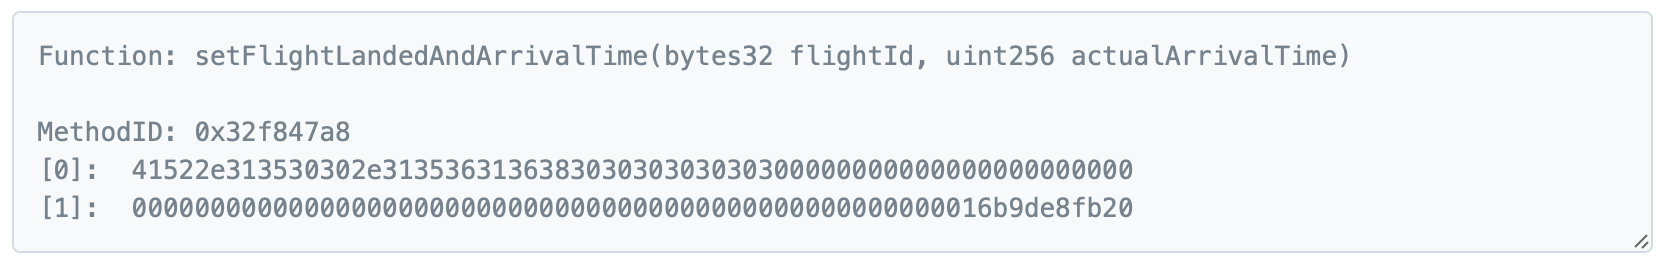
\includegraphics[width=\textwidth]{Bilder/FizzyExampleFlightLanded.png}
  \caption[Input-Daten setFlightLandedAndArrivalTime]{Input-Daten setFlightLandedAndArrivalTime \cite{FizzyFlightLanded2019}}
  \label{fig:fizzyFlightLanded}
\end{figure}

Sieht man in einem Tool wie etherscan.io in die Transaktionsliste, findet man am 28. Juni die Transaktion \texttt{0xcb63f57039f144073c4a4b45621a3c0da4593bd2185c14838d7b7e4c537f5be9}, deren Daten auch in Abbildung \ref{fig:fizzyFlightLanded} zu sehen sind. Da die tatsächliche Ankunftszeit mit umgerechnet 11:47 (GMT) weit unter der Höchstgrenze liegt, wird in diesem Fall keine Kompensation ausgezahlt.\\
Anders im Beispiel aus Abbildung \ref{fig:fizzyTrigger}, bei dem der Status auf 1 gesetzt wird, was gleichzusetzen mit einem abgeschlossenen Flug inklusive Kompensation ist.

\begin{figure}[h!]
  \centering
  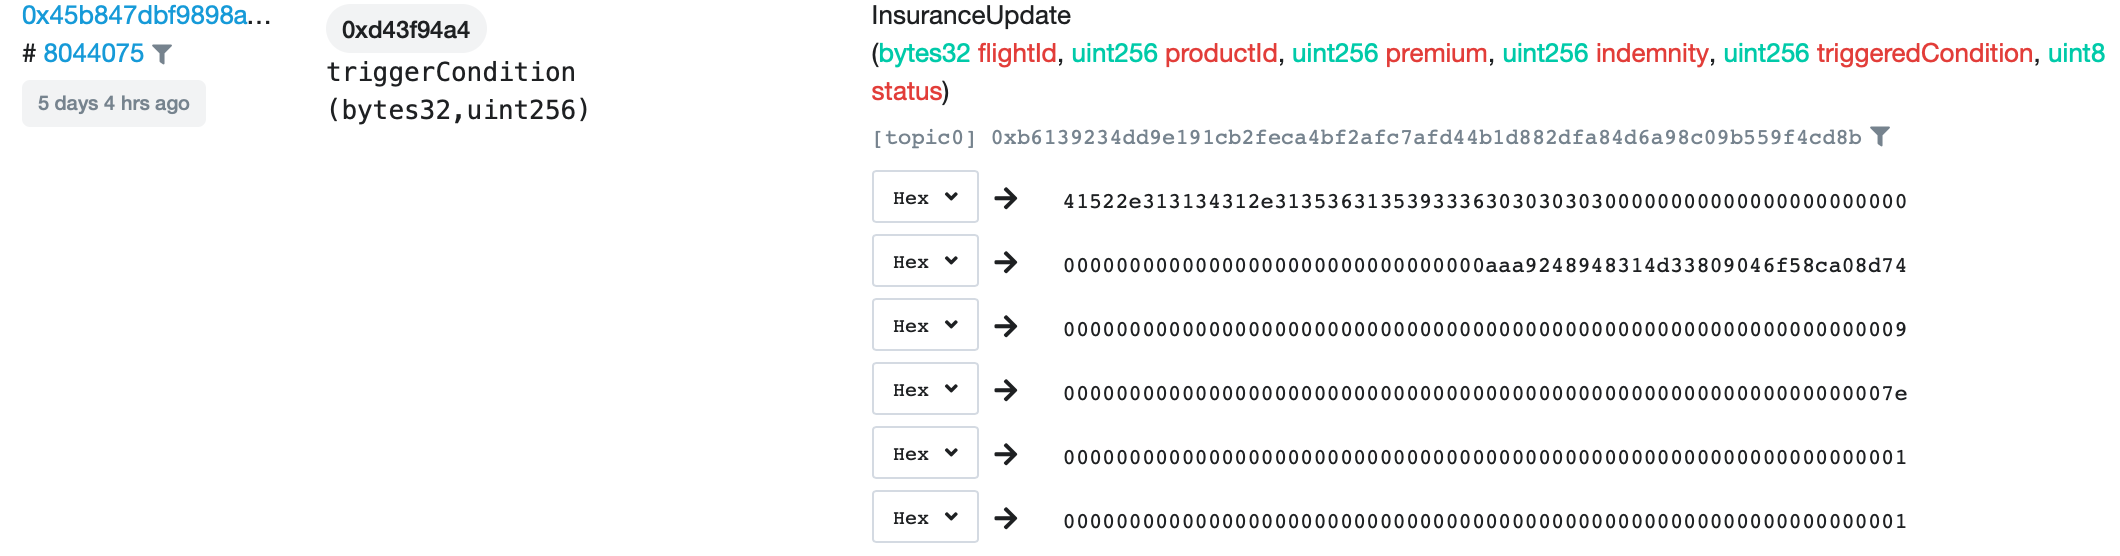
\includegraphics[width=\textwidth]{Bilder/FizzyExampleTrigger.png}
  \caption[Triggern einer Bedingung]{Triggern einer Bedingung \cite{FizzyTrigger2019}}
  \label{fig:fizzyTrigger}
\end{figure}

Fizzy ist nur eines von vielen Beispielen der Versicherungsbranche, die auf die Blockchain setzen. Es scheint so, als wäre auch hier ähnlich den Anfangsbestrebungen des B3i eher die Machbarkeit überprüft worden, anstatt alle gewohnten Prozesse auf Blockchain-Anwendungen und Smart Contracts umzustellen. Das belegen auch die Zahlen: Der alte Smart Contract umfasst ca. 20 000 Transaktionen \cite{EtherscanOldContract2019}, der neue noch nicht einmal eine dreistellige Anzahl \cite{EtherscanNewContract2019}. Dabei gilt zu berücksichtigen, dass 20 000 Einträge nicht 20 000 Versicherungen bedeutet, da mit dem Anlegen einer Versicherung und der Landung des Flugs mindestens zwei Methoden des darunterliegenden Contracts aufgerufen werden müssen. Dennoch ist die Umsetzung gelungen, da die Transparenz im Bezug auf die Bedeutung der einzelnen Parameter der Contract-Funktionen sehr positiv auffällt. So kann jeder die Abwicklung seines Fluges beobachten, ohne das persönliche Daten offengelegt werden. Trotzdem stellt sich auch hier wieder die Frage, inwiefern der Einsatz einer Blockchain-Lösung Vorteile bringt. Die Abwicklung der Kompensation kann zwar durch die eingebauten Trigger automatisch von Statten gehen, dennoch wird ein System für das Anlegen der Versicherung inklusive Datenhaltung für persönliche Daten und Zahlungsdaten benötigt. Hinzu kommen noch die Transaktionsgebühren der Ethereum Blockchain.



